\documentclass[
  amsmath,
  amssymb,
  aps,
  twocolumn,
  nofootinbib,
  nolongbibliography,
  floatfix,
]{revtex4-2}

\usepackage{bm}
\usepackage{graphicx}
\usepackage{braket}
\usepackage{xcolor}
\usepackage[colorlinks=true,allcolors=magenta]{hyperref}

\newcommand{\parens}[1]{\left ( #1 \right )}
\newcommand{\brackets}[1]{\left [ #1 \right ]}
\newcommand{\jtd}[1]{{\color{red}\textbf{JTD: #1}}}

\begin{document}
\title{Magnetic Phase Transitions in an Aperiodic Monotile}
\author{Jack Dinsmore}
\affiliation{Department of Physics, Stanford University}

\begin{abstract}
  A family of shapes known as ``einstein tiles'' has been discovered which tile the plane aperiodically. We define the Ising, XY, and Heisenberg models on the einstein tilings and compute the magnetization and susceptibility of the tiling as a function of temperature using Monte Carlo methods. This allows us to produce phase diagrams of the relationship between the critical temperature of the tiling and the dimensions of the einstein tile.
\end{abstract}

\maketitle

\section{Introduction}
The Ising model was one of the first statistical mechanics models to contain a phase transition and remains one of the only exactly solvable examples. It consists of defining a variable $s_i = \pm 1$ at every site of a lattice as a classical approximation of the up-or-down spin of a fermion. On further analogy with fermionic spins, it allows neighboring spins to interact under the classical Hamiltonian
\begin{equation}
  H = -J \sum_{\braket{ij}} s_i s_j - h \sum_i s_i
  \label{eqn:ising}
\end{equation}
where $h$ is an applied magnetic field and $\braket{ij}$ indicate neighbors. Henceforth, we'll set $h=0$. This model's phase transition is visible in the magnetization, defined as
\begin{equation}
  M = \frac{1}{N}\Braket{\sum_{i} s_i}
  \label{eqn:magnetization}
\end{equation}
where the brackets indicate a statistical average over all states, weighted by the Boltzmann factor $e^{-\beta H}$.

The phase transition occurs for the following reason. For $h=0$, the Hamiltonian displays $s_i\rightarrow -s_i$ symmetry. If the thermodynamic system explores all of phase space, then the average thermodynamic state should possess the same symmetries of the Hamiltonian so that $M=0$. However, at low temperature we also expect the system to attain the lowest possible energy, which consists of all spins up (or all spins down). Such a state has $M =\pm 1$ which violates the expectation of no magnetization. The resolution to this apparent contradiction that there exists a critical temperature $T_c$ below which energetic considerations dominate and the crystal is magnetic ($|M|>0$), and above which the symmetry of phase space dominates and the crystal is not magnetic ($M = 0$).

The phenomenon of critical temperature has been generalized to other theories. In particular, if the system's variables are arranged as a members of a field $s(\bm x)$, then the free energy may be approximated as an integral of a function of $s(\bm x)$. This approximation is called Landau Field Theory and it yields a form which is readily able to create phase transitions. Taking the Ising model as an example, we approximate the $s_i$ spins defined on discrete points $x_i$ as the field $s(\bm x)$ defined for any position $\bm x$. The original Hamiltonian contained translational, rotational, and $s\rightarrow-s$ symmetry, and therefore the free energy should as well. Expanding its integrand in powers of $s(\bm x)$ guarantees the form
\begin{equation}
F \propto -\int d^2 x \brackets{(\nabla s(\bm x))^2 + A s(\bm x)^2 + B s(\bm x)^4 + \dots}
\label{eqn:landau}
\end{equation}
where $A$ and $B$ are arbitrary constants. If $A>0$, then the integrand is minimized by setting $s(\bm x)=0$. However if $A<0$, then the average value of $s(\bm x)$ is nonzero and the crystal is magnetized. In principle, all the parameters of the model including $A$ may depend on temperature, so any theory whose $A$ crosses from positive to negative at a temperature $T_c$ contains a phase transition. 

The utility of this field theory framework is its generality. All Ising-like models are Landau field theories and are all described by Eq~\ref{eqn:landau}, meaning they have the same near-critical-point behavior. This statement is independent of the lattice or interaction strengths; it depends only on the degrees of freedom (DOFs) of the field $s$ and the dimensionality of the lattice. A particular lattice's only unique properties its its values of $A$ and $B$; i.e., the value of its critical temperature.

% The solution to a spin model depends on the lattice on which the model is defined. For example, an exact solution exists for the two-dimensional Ising model defined on the square lattice which yields an exact formula for the critical temperature. In the absence of a full solution, a series expansions in $\beta$ (valid at high temperature) or $e^{-\beta}$ (valid at low temperature) can be written for the model's thermodynamical quantities. For self-dual lattices such as the square lattice, the coefficients of the high- and low-temperature expansions are the same --- a phenomenon known as Kramers-Wannier duality \cite{kramers}. This duality leads to an analytical solution for the critical temperature even in the absence of a full solution. Even for lattices which are not self-dual, it is sometimes possible to use a similar technique to relate the series expansions of the lattice and its dual to each other. This can be done for the hexagonal lattice, for example, which is dual to the triangular lattice \cite{bhattacharjee1995fifty}.

In complicated crystals, the only available approaches to computing $T_c$ are numerical. For example, the Penrose lattice consists of two tiles which fill the two-dimensional plane aperiodically, making it difficult to model the system analytically. Ref. \cite{penrose-ising} computes magnetism as a function of temperature using numerical methods and finds that the aperiodic nature of the lattice does not affect the physics at a qualitative level, since $M(T)$ inherits most of its properties from the general Landau theory.

Recently, the first \textit{single} tile which fills the plane aperiodically has been discovered, and named the einstein tile (German for ``one stone'') (figure \ref{fig:einstein}) \cite{smith2023aperiodic}. An interesting fact about the einstein tile is that its dimensions are adjustable. The tile consists of two side lengths $a$ and $b$, and any ratio of $a/b$ leads to an aperiodic tiling except $a/b=0$, 1, or $\infty$. If we treat the spin-spin interaction as dependent on bond length, then this $a/b$ ratio represents a free parameter of the model, so that the critical temperature is a function of $a/b$. The phase diagram of $T_c(a/b)$ is therefore an intrinsic property of the einstein tiling, and more flexible than the behavior of $M(T)$.

\begin{figure}
  \centering
  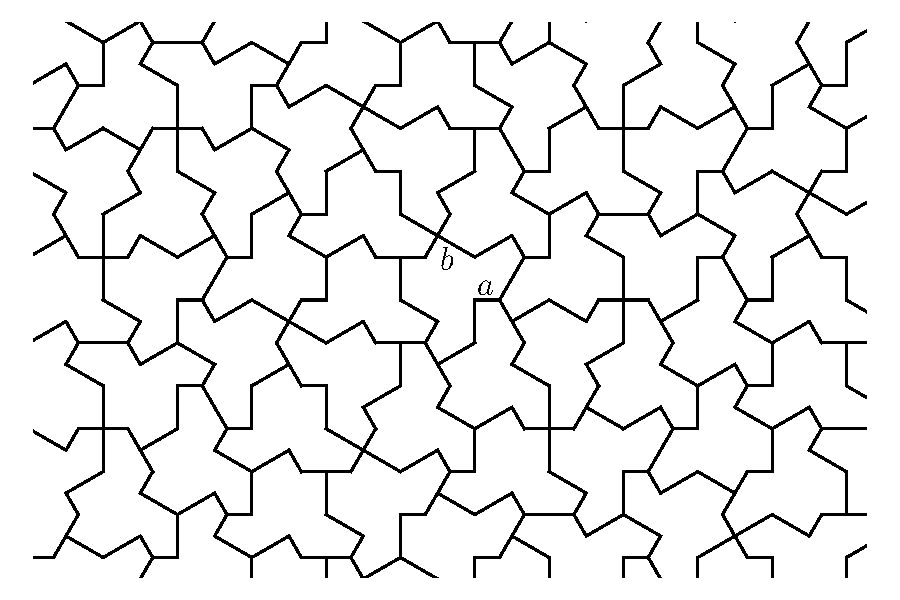
\includegraphics[width=\linewidth]{../figs/einstein.pdf}
  \caption{The einstein tiling with $b/a=\sqrt{3}$. Any other fraction $b/a$ gives a different einstein tiling}
  \label{fig:einstein}
\end{figure}

In this final project, we use numerical methods to compute the phase diagram $T_c(a/b)$ for the einstein tile under the Ising model and two similar models. The spin models are discussed in section \ref{sec:spin-models} and the numerical methods in section \ref{sec:wolff}. We also compute the phase diagram for a rectangular lattice to compare to the einstein lattice phase diagram in section \ref{sec:results}, later using this calculation to explain the one-dimensional transverse Ising model in section \ref{sec:tim}. We conclude with section \ref{sec:conclusion}.


\section{Spin models}
\label{sec:spin-models}

In addition to the Ising model Hamiltonian (Eq.~\ref{eqn:ising}), we study the XY model which consists of promoting $s_i$ to a two-dimensional unit vector defined at every lattice point. The interaction term in the Hamiltonian becomes $\bm s_i \cdot \bm s_j$. A third spin model is the Heisenberg model, which promotes $s_i$ to a three-dimensional unit vector. These models are all different in that they have progressively more spin DOFs, leading to progressively lower $T_c$. Each model also has specialized features, like the XY model's topologically protected vortices and the Heisenberg model's pseudo-phase transition \cite{tomita2014finite}, but these are beyond the scope of this report.

A fourth spin model is the Transverse Ising Model (TIM), which consists of replacing $s_i$ in Eq.~\ref{eqn:ising} with the Pauli matrices $\bm \sigma_i$ and $\bm \sigma_j$ and interpreting the result as a quantum Hamiltonian. A simple proof (section \ref{sec:tim}) shows that the TIM is equivalent to a classical Ising model, so critical temperatures for all four of these models can be found using the same techniques.

Beyond the magnetization $M$, another interesting property of a spin model is its susceptibility $\chi = \frac{dM}{dh}$. Even in a model which sets $h=0$, $\chi$ can be achieved by explicitly differentiating Eq.~\ref{eqn:magnetization}, including the $e^{-\beta H}$ weight in the average. This differentiation results in the zero-$h$ limit of
\begin{equation}
  \chi = \frac{\partial M}{\partial h} = \frac{1}{N}\Braket{\sum_i(s_i - M)^2}.
\end{equation}
This is a special case of the fluctuation-dissipation theorem, which states that a driving field $h$ causes fluctuations in the driven variable $M$ which are proportional to the susceptibility $\chi$. A spin model is most susceptible to magnetic field near $T_c$, because the presence of a magnetic field changes the value of $T_c$ and therefore can greatly change the magnetization of a system near $T_c$. Thus the susceptibility diverges at $T_c$ and otherwise falls off to zero.


\section{Cluster Monte Carlo Methods: the Wolff Algorithm}
\label{sec:wolff}

To find the critical temperature of the einstein lattice, we must numerically compute the ensemble average of Eq.~\ref{eqn:magnetization}. This average is extremely expensive to compute because the number of states in the ensemble is $2^N$ for the Ising model. However, approximate results can be obtained by computing the sum over a much smaller, random selection of states $K$. This approximation technique is called a Monte Carlo method.

The method of selecting states for $K$ is critical to the accuracy of a Monte Carlo method. It needs to add states $\psi$ to $K$ with some probability $P(\psi)$ which prefers states that are representative of the full ensemble, otherwise the convergence of the ensemble average will be poor. Many states are not representative, making it difficult to find a new state $\psi$ which has high enough $P(\psi)$ to be added to $K$. One way to resolve this problem is to make $\psi$ very similar to a state $\phi$ already in $K$ --- a technique known as a Markov Chain Monte Carlo method (MCMC). Assuming $\phi$ is representative of the ensemble, then $\psi$ is also likely to be represented by the ensemble. We then add $\psi$ to $K$ with some probability $P(\phi \rightarrow \psi)$.

For an MCMC to be correct, $P(\phi \rightarrow \psi)$ must be reversible, meaning that the probability to go from $\phi$ to $\psi$ must be equal to the probability to go from $\psi$ to $\phi$. This condition is necessary to prevent $K$ from getting stuck in an unrepresentative region of phase space. The probability to go from $\phi$ to $\psi$ is the probability for the MCMC to be at state $\phi$ in the first place times the probability to switch to $\psi$. Thus, reversibility requires
\begin{equation}
  P(\phi \rightarrow \psi)P(\phi) = P(\psi \rightarrow \phi)P(\psi)
  \label{eqn:detailed-balance}
\end{equation}

There are many methods of generating new states, but the one we will use in this paper is the Wolff algorithm, which is known to converge well near the critical temperature \cite{wolff1989collective}. The algorithm generates a new state $\psi$ by probabilistically choosing a cluster of spins and then flipping all the spins at once. The cluster starts the cluster at a random location $i$. It then adds each neighbor $j$ to the cluster with probability
\begin{equation}
  P(i,j) = 1 - \exp\parens{\mathrm{min}\left[0, 2\beta s_i s_j \right]}.
  \label{eqn:wolff-algo}
\end{equation}
For every spin $j$ which was added to the cluster, it then uses the same equation to assign $j$'s neighbors to the cluster until every neighbor has been rejected. At that point, the cluster's spins are flipped to form the new state $\psi$. Ref.~\cite{wolff1989collective} confirms that Eq.~\ref{eqn:wolff-algo} satisfies the reversibility constraint Eq.~\ref{eqn:detailed-balance} and therefore is a good MCMC.

For the XY and Heisenberg models, Eq.~\ref{eqn:wolff-algo} must be modified to handle vector-valued spins. The approach is to choose a random unit vector $\bm r$ as a direction against which to compare to spins, so that
\begin{equation}
  P(i,j) = 1 - \exp\parens{\mathrm{min}\left[0, 2\beta J (\bm r \cdot \bm s_i)(\bm r \cdot \bm s_j) \right]}.
\end{equation}
For consistency, we keep $\bm r$ the same throughout the cluster, but for the next cluster we re-draw a new $\bm r$.

% A third and final extension is necessary to the Wolff algorithm in order to handle quantum spin models. As mentioned above, the TIM in two dimensions is equivalent to the Ising model in three dimensions where interaction strengths $J$ are very strong in the new direction. We could therefore stack many two-dimensional crystals to form a three-dimensional crystal on which we run the Wolff algorithm, but this is inefficient because the large $J$ along the third axis will make the clusters grow large in this direction. Ref.~\cite{blote2002cluster} speeds up the process by analytically computing the behavior of the Wolff algorithm along the third axis in the limit of large $J$. The classical Wolff algorithm can then be run on the two-dimensional lattice while the spins on the third axis are set according to this analytical result.

\section{Results}
\label{sec:results}

We implemented the Wolff algorithm with a custom code base\footnote{\url{https://github.com/jack-dinsmore/quasing-model}} and executed it for a variety of spin models and crystals. Except when stated otherwise, we used a finite-size lattice with initial conditions of random spins. Magnetization $M$ and susceptibility $\chi$ measurements were collected every 16 cluster flips to prevent autocorrelation. 10,000 $M$ and $\chi$ measurements were made when $M$ was small, and when $M$ was large we made 1,000 measurements because the algorithm was found to be more stable for $T< T_c$.

The upper left panel of Figure \ref{fig:square} shows the magnetization $M$ and susceptibility $\chi$ of the Ising, XY, and Heisenberg models executed on a square lattice with periodic boundary conditions as a function of the temperature $T$. The magnetization drops rapidly near $T_c$, shown as vertical dotted lines, though the drop is not immediate due to finite-size effects. The XY and Heisenberg models have substantially lower $T_c$ due to the increased DOFs of the spin system. Furthermore, $M$ approaches its low-temperature limit of 1 linearly for the Heisenberg and XY models, while the approach is exponential for the Ising model. This is a qualitative difference between the Ising and XY models.

\begin{figure*}
  \centering
  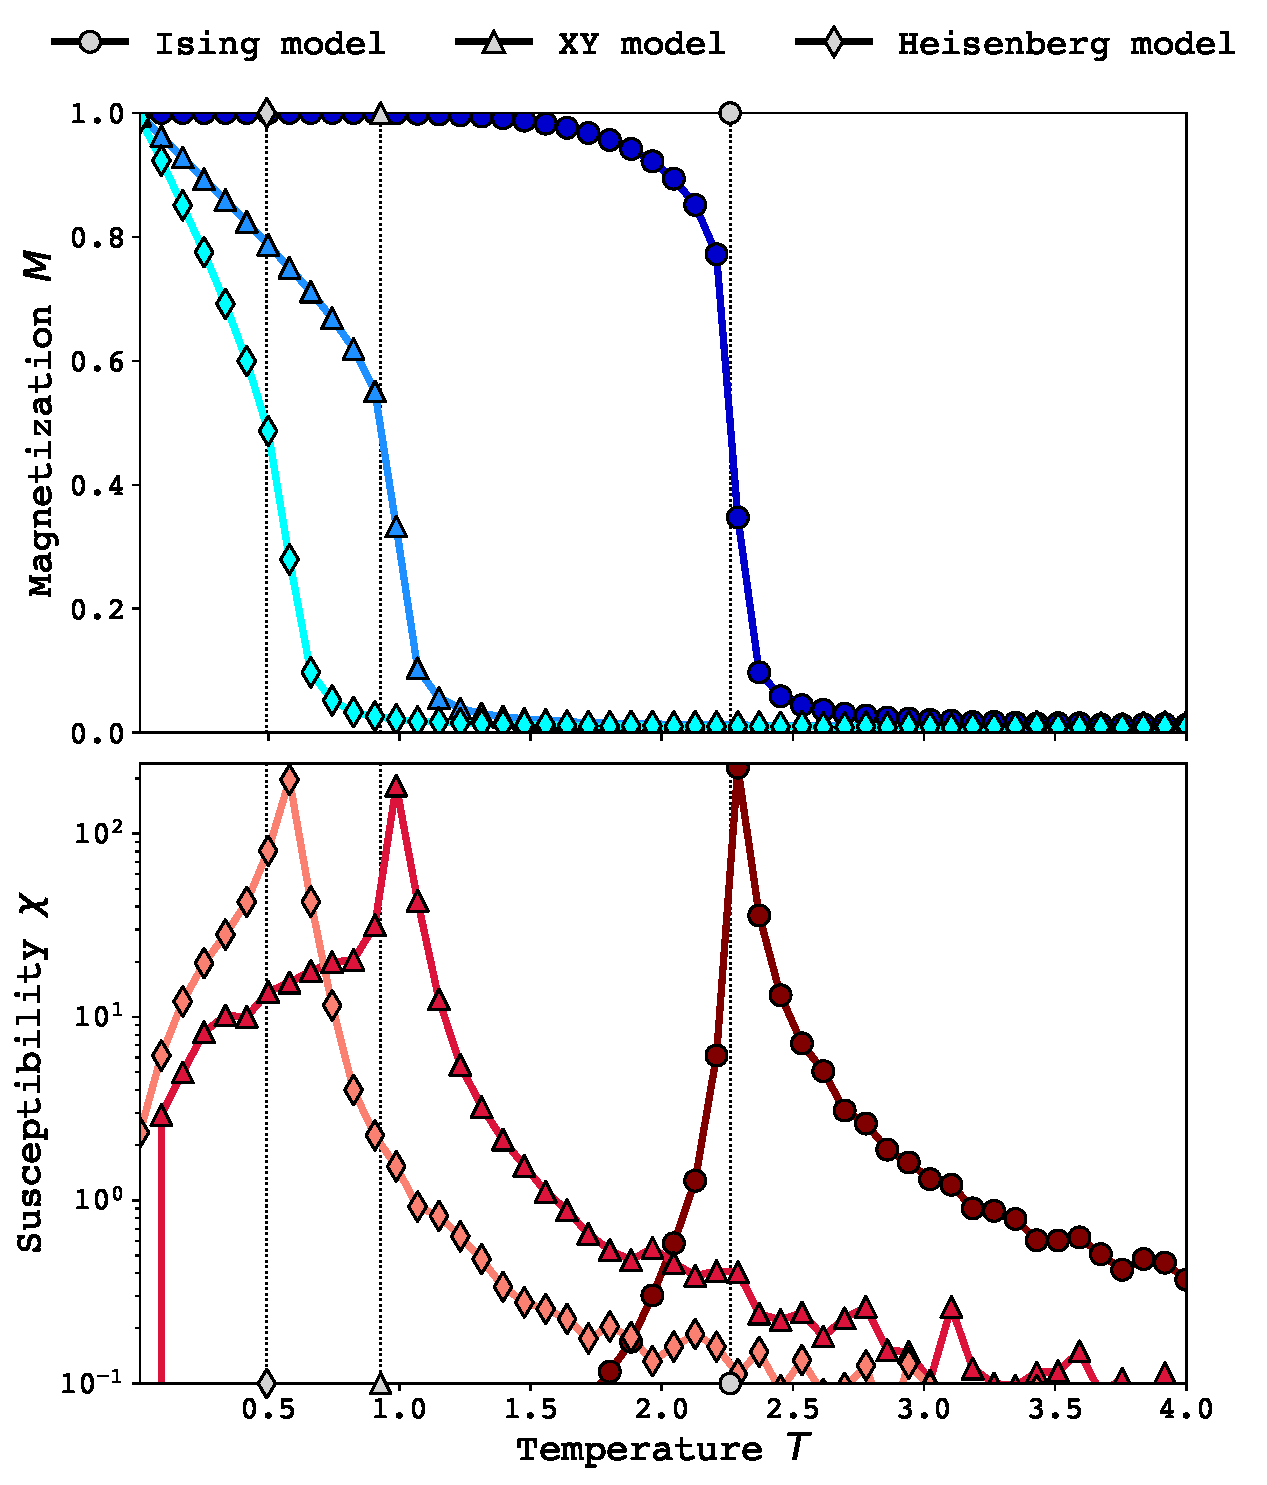
\includegraphics[width=0.49\linewidth]{../figs/square.pdf}\hfill
  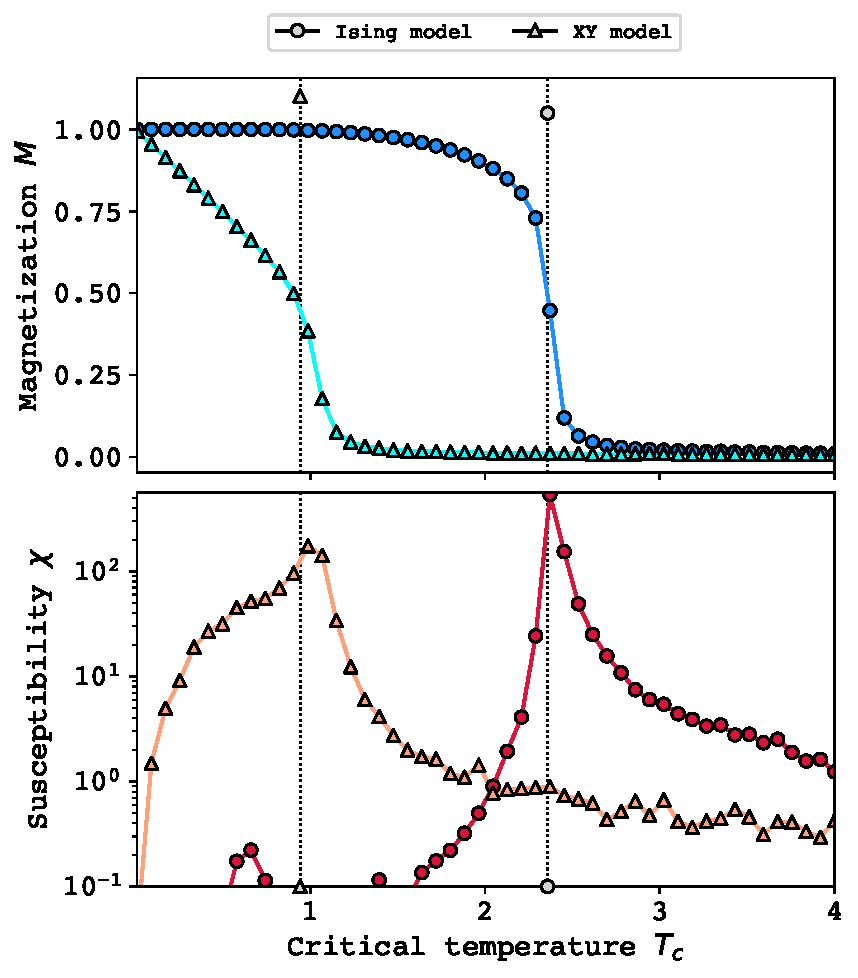
\includegraphics[width=0.49\linewidth]{../figs/penrose.pdf}
  \caption{Magnetization and susceptibility as a function of $T_c$ under the Ising, XY, and Heisenberg models. \textit{Left}: A square lattice with $N=128^2=16,384$ sites. \textit{Right}: A Penrose lattice with $N=21,316$ sites. The three spin models yield very different predictions but the two crystals are similar due to their field theory explanation.}
  \label{fig:square}
\end{figure*}

The susceptibility $\chi$ in the bottom left panel produces a maximum at $T_c$. For the Ising model, the decay to zero more is more rapid on the low-temperature side than high-temperature, though the reverse is true for the XY and Heisenberg models. For an infinite lattice, the peak in $\chi$ will be likewise infinite, though here it is blunted by finite $N$.

For the sake of approximating $T_c$, we take the $T$ point at which the steepest line tangent to the $M(T)$ curve intersects $M=0.5$. The critical temperatures obtained from this approximation are shown in table \ref{tab:tc}. These temperatures are very close to the true values known for the square lattice: For the Ising model, the Onsager solution gives $T_c = \frac{2}{\ln(1 + \sqrt{2})} \approx 2.2691$ in units where $J=k_B=1$, and for the XY model larger lattice MCMC methods give $T_c \approx 0.8816$. The $N\rightarrow \infty$ Heisenberg model does not have a true phase transition, but this fact is difficult to verify in a lattice of finite size, which never have true phase transitions in any case. 
\begin{table}
  \centering
  \begin{tabular}{c|ccc}
    \hline \hline
    & Square & Penrose & Einstein\\ \hline
    Ising & 2.26 & 2.36 & 0.396\\
    XY & 0.928 & 0.943 & 0.130\\
    Heisenberg & 0.493 & 0.462 & 0.0548\\ \hline \hline
  \end{tabular}
  \caption{Critical temperatures $T_c$ for the Ising, XY, and Heisenberg models defined on the square and Penrose lattices in units where $J = k_B = 1$. These values are very close to the true values (see text). Also shown are $T_c$ for the einstein lattice with $\eta=-\frac{1}{3}$ as depicted in figure \ref{fig:einstein}.}
  \label{tab:tc}
\end{table}

To demonstrate that the $M(T)$ relationship is not strongly dependent on the lattice, we also compute the same quantities for the Penrose lattice, shown in the right two panels of figure \ref{fig:square}. The same limiting behavior of $\chi$ and $M$ is present in both crystals, with slight changes in the steepness of the curves due to the difference in $N$. The major difference between the two is the actual value of $T_c$, which is slightly higher for Penrose (table \ref{tab:tc}).

The square lattice can be stretched into a rectangular lattice by allowing the horizontal and vertical bonds to differ in length. Assigning different interaction strengths $J_1$ and $J_2$ to the two bond lengths gives a free parameter $J_1/J_2$. If we let $J \propto \ell^{-2}$ where $\ell$ is the bond length, then the phase diagram is further parameterized by the length ratio $a/b$.

Let us define the anisotropy $\eta$ of the lattice as 
\begin{equation}
  \frac{a}{b} = \tan\brackets{\frac{\pi}{4}\parens{1+\eta}},\qquad \eta = \frac{4}{\pi}\tan^{-1}\parens{\frac{a}{b}}-1.
  \label{eqn:anisotropy}
\end{equation}
We fix the product of the lengths $ab=1$, so that 
\begin{equation}
  a^2 = \tan\brackets{\frac{\pi}{4}\parens{1+\eta}},\qquad b^2 = \tan\brackets{\frac{\pi}{4}\parens{1-\eta}}.
\end{equation}
Then $\eta \in (-1,1)$ and $\eta=0$ implies $a=b$. For the square lattice in particular, rotational symmetry guarantees that the phase diagram $T_c(\eta)$ is symmetric under $a\leftrightarrow b$, or $\eta \rightarrow -\eta$.

\begin{figure}
  \centering
  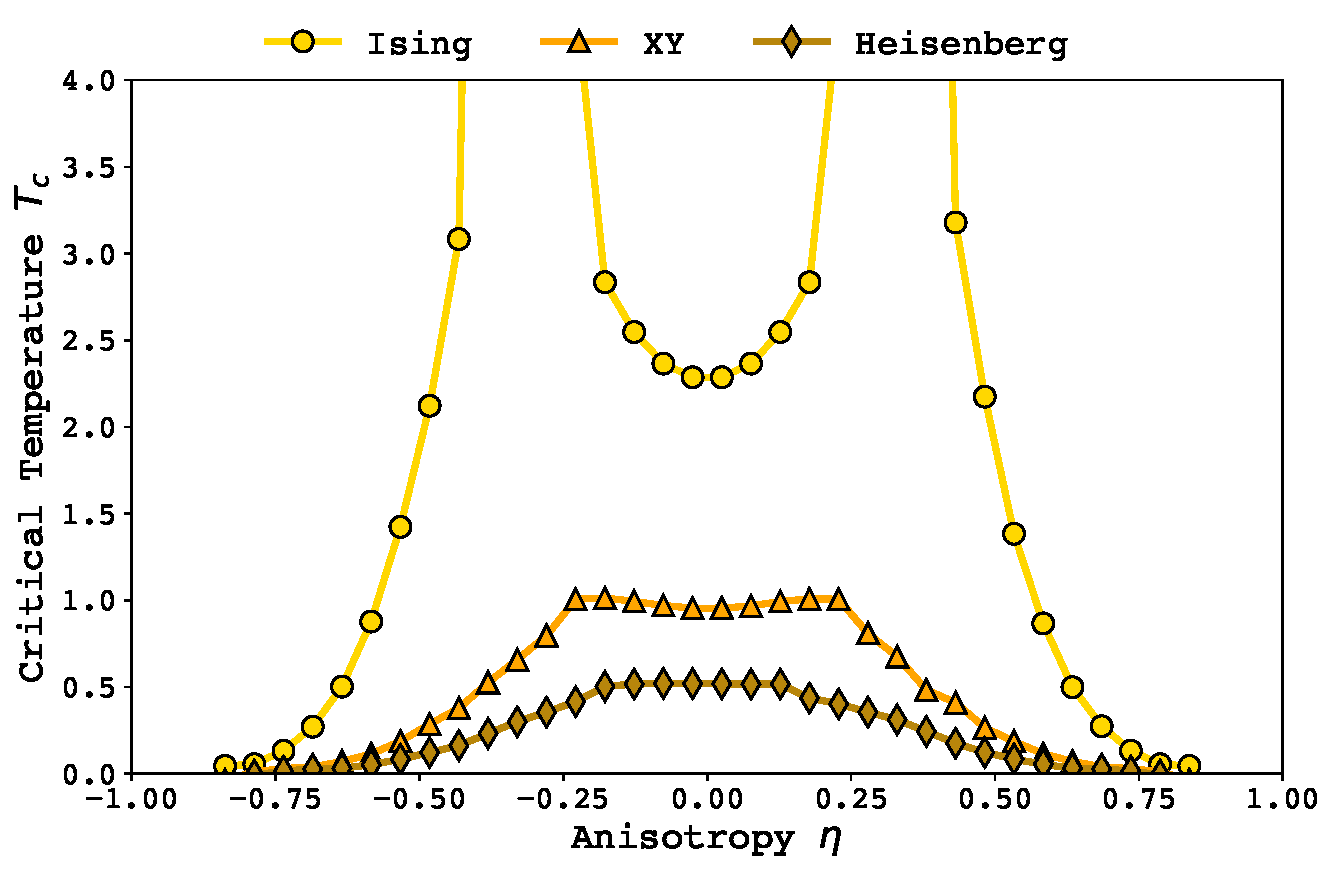
\includegraphics[width=\linewidth]{../figs/rect-phase.pdf}
  \caption{The phase diagram of the rectangular lattice as a function of the anisotropy $\eta$, where $\eta = 0$ is the square lattice. This function is even due to the rotational symmetry of a rectangular lattice.}
  \label{fig:rect-phase}
\end{figure}

Figure \ref{fig:rect-phase} shows $T_c$ as a function of $\eta$ for the rectangular lattice under the Ising, XY, and Heisenberg models. As expected, the result is symmetric around $\eta \rightarrow -\eta$. Anisotropy increases $T_c$ near $\eta = 0$ in the Ising and XY models, though this trend turns over at some $\eta$ to achieve $T_c\rightarrow 0$ in the limit as $\eta \rightarrow \pm 1$. For the Ising model, the turnover occurs at $\eta\approx \pm 0.625$ after which $T_c$ falls to zero rapidly. For the XY model, the maximum value of $T_c$ occurs at $\eta \approx \pm 0.362$, which is half the turnover $\eta$ of the Ising model. However, $T_c$ falls only slowly until $\eta \approx 0.5$, after which $T_c$ drops to zero.

\begin{figure}
  \centering
  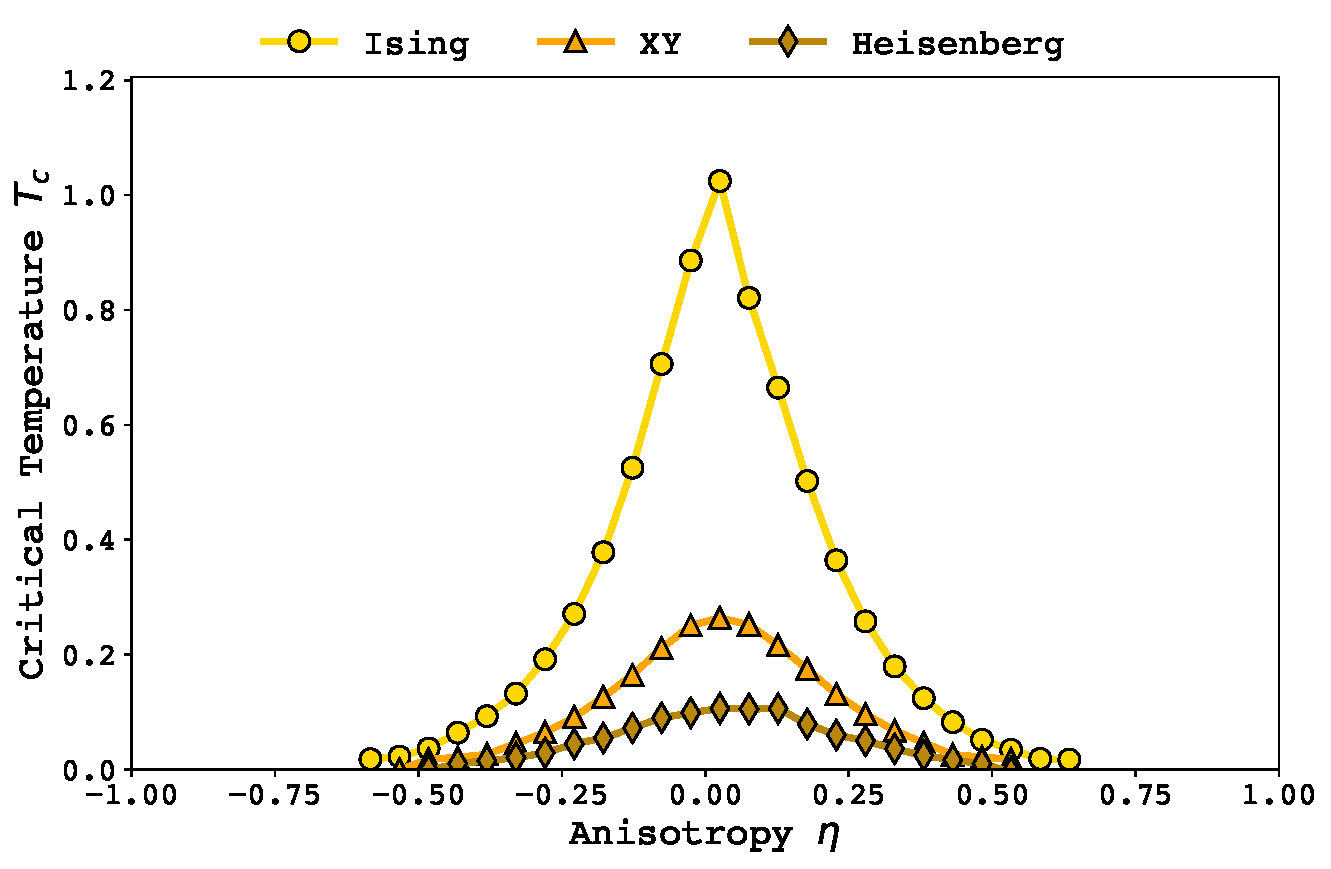
\includegraphics[width=\linewidth]{../figs/einstein-phase.pdf}
  \caption{The phase diagram of the einstein tiling as a function of the anisotropy $\eta$. The temperature is even after a shift in $\eta$.}
  \label{fig:einstein-phase}
\end{figure}

For the Heisenberg model, $T_c$ is maximal at $\eta=0$, though it remains constant to within a fraction of a percent until $\eta \approx 1/3$ at which point $T_c$ begins to decrease. All of these turnover values of $\eta$ may depend on the length $L$ of the lattice. In the $N\rightarrow \infty$ limit, a series expansion approach may help to reveal why these turnover values occur and how they depend on the number of DOFs of the spin model.

A similar procedure shows the phase diagram for the einstein tiling with $N=7,047$ sites, where $a$ and $b$ are now the two lengths shown in figure \ref{fig:einstein}. The phase diagram is shown in figure \ref{fig:einstein-phase}. In this case, anisotropy decreases $T_c$ in every model so that the maximum anisotropy occurs near $\eta = 0$, which corresponds to a regular lattice. The $T_c$ of the lattice depicted in figure \ref{fig:einstein}, which has $\eta = -1/3$, is given in table \ref{tab:tc}. Critical temperatures for all $\eta$ are much lower than for any other crystals studied here because of the relatively low coordination number of each site in the einstein tiling. Many sites are connected to the minimum two bonds in einstein whereas the Penrose and square model had average coordination number of 4 in the $N\rightarrow \infty$ limit. Since more connected lattices have stronger spin interactions, this is qualitatively similar to fixing $J$. Dimensional analysis requires that the critical value of any crystal is proportional to $\beta_c J = J/T_c$ so that increasing $J$ implies increasing $T_c$.

If $\eta$ is shifted by some amount $\eta \rightarrow \eta - x$, then $T_c(\eta)$ possesses $\eta\rightarrow -\eta$ symmetry for the einstein tiling. This is surprising because $\eta$ and $-\eta$ correspond to completely different lattices, suggesting the presence of some greater symmetry in the einstein tiling which has not yet been remarked. Other models defined on the einstein tiling do not always contain this symmetry. The shift value $x$ is 0.029 for the Ising model, 0.052 for the XY model, and 0.033 for the Heisenberg model, though these shift values may depend on both numerical fluctuations of the MCMC and on the finite $N$ used.

\section{Transverse Ising Model}
\label{sec:tim}

Quantum mechanical models such as the TIM cannot in general be represented by the same formalism as a classical model. However the the TIM is a special case: A $d$-dimensional TIM is equivalent to a $d+1$-dimensional anisotropic Ising model, as first discovered in Ref.~\cite{schultz64two}. We will prove this in the case of $d=1$. To see this, consider the quantum partition function
\begin{equation}
  Z = \mathrm{Tr}\parens{e^{-\beta H}}.
  \label{eqn:quantum-partition}
\end{equation}
For clarity, the Hamiltonian for the TIM is
\begin{equation}
  H = -J \sum_{\braket{ij}}\bm \sigma_i \cdot \bm \sigma_j - h \sum_i\sigma_i^3
\end{equation}
where $\bm \sigma_i$ is the spin operator (a vector of Pauli matrices) for site $i$. Since $H$ is time-independent and therefore self-commuting, this is 
\begin{equation}
  \begin{split}
    Z =& \mathrm{Tr}\parens{e^{-\epsilon H}\dots e^{-\epsilon H}}\\
     =& \sum_{\psi_0\in\mathcal{H}}\bra{\psi_0}e^{-\epsilon H}\parens{\sum_{\psi_1\in\mathcal{H}}\ket{\psi_1}\bra{\psi_1}}\times\dots\\
     &\times e^{-i\epsilon H}\parens{\sum_{\psi_n\in\mathcal{H}}\ket{\psi_n}\bra{\psi_n}}\ket{\psi_0}
  \end{split}
\end{equation}
where $\ket{\psi_a}$ indicates a quantum state in the Hilbert space $\mathcal{H}$. In the second line we just inserted the identity many times as well as the definition of the trace. The number $n$ is set such that $\epsilon n = \beta$ to satisfy Eq.~\ref{eqn:quantum-partition}. Setting $\epsilon$ sufficiently low, we can expand the exponential to first order in $\epsilon$:
\begin{equation}
  \begin{split}
    Z =& \sum_{\{\psi\}}\bra{\psi_0}(1 - \epsilon H)\ket{\psi_1}\bra{\psi_1}\times\dots\\
    &\times (1 - \epsilon H)\ket{\psi_n}\braket{\psi_n|\psi_0}.
  \end{split}
  \label{eqn:partition-simplified}
\end{equation}
where we have collapsed all the sums into one. In an orthonormal basis where $\braket{\psi_a|\psi_b} = \delta_{ab}$, the only $\mathcal{O}(\epsilon^0)$ term in Eq.~\ref{eqn:partition-simplified} is for all $\ket{\psi_a}$ equal. So to order $\mathcal{O}(\epsilon)$,
\begin{equation}
  \begin{split}
    Z &= 1 - \epsilon\sum_{a\neq b}\braket{\psi_a|H|\psi_b}\\
    Z &= 1 - \epsilon\sum_{a\neq b}\Braket{\psi_a|-J\sum_{\braket{ij}}\bm \sigma_i \cdot \bm \sigma_j - h\sum_i\sigma_i^3|\psi_b}
  \end{split}
\end{equation}
As our basis, we may take the wavefunctions $\ket{s_1 s_2 \dots s_N}$ where $s_i$ indicates the sign of the spin of site $i$ and there are $N$ sites. Explicit calculation verifies that $\braket{s_is_j|\bm \sigma_i \cdot \bm \sigma_j|s_i's_j'}=\delta_{s_i,s_j}\delta_{s'_i,s'_j}$. We sum over the $s'$ spins and replace the $s$ Kronecker delta with $s_i s_j$, which is equal to $\delta_{s_i,s_j}$ shifted by a constant. Likewise, $\braket{s|\sigma^3|s'}=\delta_{s,s'}\sim ss'$. Expressing $\ket{\psi_a}=\ket{s_1 s_2 \dots s_N}$ and $\ket{\psi_b}=\ket{s'_1 s'_2 \dots s'_N}$, we get
\begin{equation}
  Z = 1 - \epsilon\sum_{\{s\},\{s'\}} \brackets{-J\sum_{\braket{ij}} s_is_j - h\sum_is_i s'_i}.
\end{equation}
Since this expression is order $\epsilon$, we may write it as an exponential:
\begin{equation}
  \begin{split}
    Z &= \sum_{\{s\},\{s'\}} e^{-K}.\\
    K &= -\epsilon J\sum_{\braket{ij}}\bm s_is_j +\frac{1}{2}\ln(\epsilon h)\sum_is_i s'_i.
  \end{split}
\end{equation}

If we stack the $s$ and $s'$ spins into a square grid, then this is the classical partition function of a square Ising model, with different vertical and horizontal interaction strengths. The anisotropy is very high: $\eta \sim 1 - C\sqrt{\epsilon}$ for some constant $C$.

We have already computed the behavior of the two-dimensional classical Ising model; according to figure \ref{fig:rect-phase}, $T_c\rightarrow 0$ as $\eta \rightarrow 1$, so that the critical temperature of the TIM is zero. This is a qualitative difference between the TIM and the classical Ising model; in the classial model, the only one of the two minima of the free energy must be occupied, forcing the system to choose either $M=+1$ or $M=-1$. In the quantum model both can be simultaneously occupied, with zero-energy fermion-like domain walls separating the two. Thus, the ordered phase has magnetization $M=0$ which cannot occur in the classical case.

\section{Conclusion}
\label{sec:conclusion}
After an introduction to phase transitions in classical spin-like models, first in the case of the Ising model and then in the general case of a Landau field theory, we solve the Ising, XY, and Heisenberg models on a rectangular lattice and the aperiodic Penrose and einstein tilings.

The magnetization and susceptibility as a function of temperature were discussed and shown to be dramatically different between the models, though similar for different crystals. This was explained as a consequence of the Landau field theory explanation for phase transitions, which predicts that the behavior of a theory is sensitive to the number of degrees of freedom of the spin field and less to the structure of the lattice.

Phase diagrams of the critical temperature as a function of the lattice anisotropy were shown; these are not predicted by Landau field theory and are therefore less theoretically constrained.  Anisotropy was seen to increase the critical temperature of the square lattice but decrease the critical temperature of the einstein tiling. The rectangular lattice achieved maximum critical temperature at model-dependent ``turnover values'' of anisotropy, and the einstein tiling displayed unexpected symmetry after a model-dependent shift in the anisotropy. Understanding either of these features may require deeper investigation.

Finally, we introduced a quantum Ising model --- the Transverse Ising model (TIM) --- and showed that the one-dimensional TIM it is equivalent to a two-dimensional classical anisotropic Ising model. We used our two-dimensional Ising model calculations to discuss the properties of the TIM and qualitatively contrasted the TIM with the classical models investigated here.

\bibliography{cmt.bib}

\end{document}